\documentclass[12pt,a4paper]{article}

\usepackage[utf8]{inputenc}
\usepackage{amsmath, amssymb, amsthm}
\usepackage{graphicx}
\usepackage{float}
\usepackage{booktabs}
\usepackage{tabularx}
\usepackage{siunitx}
\usepackage{hyperref}
\usepackage{bm}
\usepackage{natbib} % or biblatex if you prefer
\bibliographystyle{apa} % set APA style

\title{Time Series Clustering Using Simulated Data}
\author{Rasika Dilhani}
\date{\today}


\begin{document}
	\maketitle
	
\section{Introduction}
Time series analysis provides a framework for characterizing the structural properties of data and its random variation. In this study, we conduct a simulation experiment to examine the features of ordinal patterns within ARMA (Autoregressive Moving Average) processes. To do this, we use simulated data, also known as synthetic series, which are generated from specified time series models. Simulation plays a main role in time series research, as it facilitates the assessment of statistical properties, the construction of confidence intervals for model parameters, and the exploration of potential future scenarios. Furthermore, simulation methods are computationally accessible,  as most standard statistical distributions can be generated directly through established algorithms. To explore the features of ordinal patterns, we replicate the experiment under two different sample sizes. The aim was to investigate how different ARMA parameter settings influence the stochastic properties of the resulting time series data, particularly in terms of entropy, complexity, and other statistical features.

	
\section{ARMA model}
In this study, simulated datasets are generated for clustering time series using ordinal patterns. The base random model for sampling is the normal distribution: $\bm X=(X_1,X_2,\dots,X_n)$, with $X_i \sim N(\mu, \sigma^2)$. Here, the mean parameter varies as $\mu \in \{-1, 0, 1\}$. For investigating more complex dynamics, simulated time series are constructed using autoregressive moving average (ARMA) models, a central class of models for representing stationary processes.

\subsection{The Backward Shift (Lag) Operator}

The backward shift (or lag) operator $\mathbf{B}$ is defined as $\mathbf{B} x_t = x_{t-1}$. By repeated application, this yields $\mathbf{B}^n x_t = x_{t-n}$. This compact notation is fundamental in expressing ARMA models and related difference equations.

\subsection{ARMA Model Specification}

Let $\{x_t\}$ denote a real-valued time series. An ARMA($p,q$) process can be written as:
\begin{equation}
	x_t = \alpha_1 x_{t-1} + \alpha_2 x_{t-2} + \dots + \alpha_p x_{t-p} + w_t + \beta_1 w_{t-1} + \beta_2 w_{t-2} + \dots + \beta_q w_{t-q},
	\label{eq:arma}
\end{equation}
where $\{w_t\}$ is a white noise sequence.

Using the lag operator, the above model can be expressed more compactly as:
\begin{equation}
	\theta_p(\mathbf{B}) x_t = \phi_q(\mathbf{B}) w_t,
	\label{eq:arma_polynomial}
\end{equation}
where $\theta_p(\mathbf{B}) = 1 - \alpha_1 \mathbf{B} - \alpha_2 \mathbf{B}^2 - \cdots - \alpha_p \mathbf{B}^p$ and $\phi_q(\mathbf{B}) = 1 + \beta_1 \mathbf{B} + \cdots + \beta_q \mathbf{B}^q$.

\section{Parameter Settings and Data Generation}

To systematically analyze time series structure via entropy and complexity, we define a comprehensive grid of ARMA model configurations. The following models and coefficient settings are considered:

\begin{table}[h!]
	\centering
	\begin{tabular}{llllll}
		\toprule
		\textbf{Type} & \textbf{Model} & $\alpha_1$ & $\alpha_2$ & $\beta_1$ & $\beta_2$ \\
		\midrule
		AR(1)      & AR1\_M1  & 0.8   &      &      &      \\
		& AR1\_M2  & 0.1   &      &      &      \\
		& AR1\_M3  & -0.8  &      &      &      \\
		& AR1\_M4  & -0.1  &      &      &      \\
		AR(2)      & AR2\_M1  & 0.1   & 0.8  &      &      \\
		& AR2\_M2  & -0.8  & 0.1  &      &      \\
		& AR2\_M3  & 0.1   & -0.8 &      &      \\
		& AR2\_M4  & -0.8  & -0.1 &      &      \\
		MA(1)      & MA1\_M1  &       &      & 0.8  &      \\
		& MA1\_M2  &       &      & 0.1  &      \\
		& MA1\_M3  &       &      & -0.8 &      \\
		& MA1\_M4  &       &      & -0.1 &      \\
		MA(2)      & MA2\_M1  &       &      & 0.1  & 0.8  \\
		& MA2\_M2  &       &      & -0.8 & 0.1  \\
		& MA2\_M3  &       &      & 0.1  & -0.8 \\
		& MA2\_M4  &       &      & -0.8 & -0.1 \\
		ARMA(1,1)  & ARMA11\_M1 & 0.8 &      & 0.8  &      \\
		& ARMA11\_M2 & 0.1 &      & 0.1  &      \\
		& ARMA11\_M3 & -0.8 &     & -0.8 &      \\
		& ARMA11\_M4 & -0.1 &     & -0.1 &      \\
		ARMA(2,2)  & ARMA22\_M1 & 0.1 & 0.8  & 0.1  & 0.8  \\
		& ARMA22\_M2 & -0.8 & 0.1 & -0.8 & 0.1  \\
		& ARMA22\_M3 & 0.1 & -0.8 & 0.1  & -0.8 \\
		& ARMA22\_M4 & -0.8 & -0.1 & -0.8 & -0.1 \\
		\bottomrule
	\end{tabular}
	\caption{Models and parameter sets for AR(1), AR(2), MA(1), MA(2), ARMA(1,1), and ARMA(2,2). Empty cells indicate omitted parameters.}
\end{table}


For each model type and specified parameterization:
\begin{itemize}
	\item Embedding dimension $D=3$ is used for ordinal pattern analysis.
	\item Sample sizes: $n \in \{500, 1000\}$.
	\item For each parameter configuration and each sample size, $R=100$ independent time series are simulated.
	\begin{itemize}
	\item For every time series, both permutation entropy ($H$) and statistical complexity ($C$) are computed.
	\item Each set of $(H, C)$ results is visualized: the $(H, C)$  pairs are plotted in the entropy-complexity plane, incorporating boundary curves and using axis splits suitable to each model class and time series length.
	\end{itemize}
	\item For further insight, density plots grouped by sample size illustrate the distribution of points.
	\item For each model class, four subplots (corresponding to four specific parameter combinations) are combined into one grid, yielding six grids (one per model type) for a total of $6 \times 4$ subplots.
\end{itemize}

The simulation design provides systematic coverage of AR, MA, and ARMA structures, supporting robust clustering analysis of ordinal pattern features in both short ($n=500$) and moderate ($n=1000$) time series settings. Visualization strategies enable both direct comparisons between parameterizations and analysis of overall model class behavior in the entropy-complexity space.

\section{Results and Discussion}

To evaluate the effectiveness of ordinal pattern features for time series clustering, simulation experiments were conducted with ARMA processes across a comprehensive grid of parameters. Specifically, the autoregressive (AR) and moving average (MA) coefficients were varied over the sets:
\[
\text{AR} \in \{-0.8,\ -0.1,\ 0.8,\ 0.1 \}
\]
\[
\text{MA} \in \{-0.8,\ -0.1,\ 0.8,\ 0.1 \}
\]
For each combination of AR and MA parameters, a time series was simulated and analyzed using ordinal patterns. The simulation loop systematically covered all grid points, ensuring a variety of dynamic behaviors and noise structures.

Figures~\ref{fig:HC AR(1)} to~\ref{fig:HC ARMA(22)}  display entropy–complexity $(H \times C)$ plane scatter plots derived from simulated data, covering diverse AR and MA parameter combinations and sample sizes.

\begin{figure}[H]
	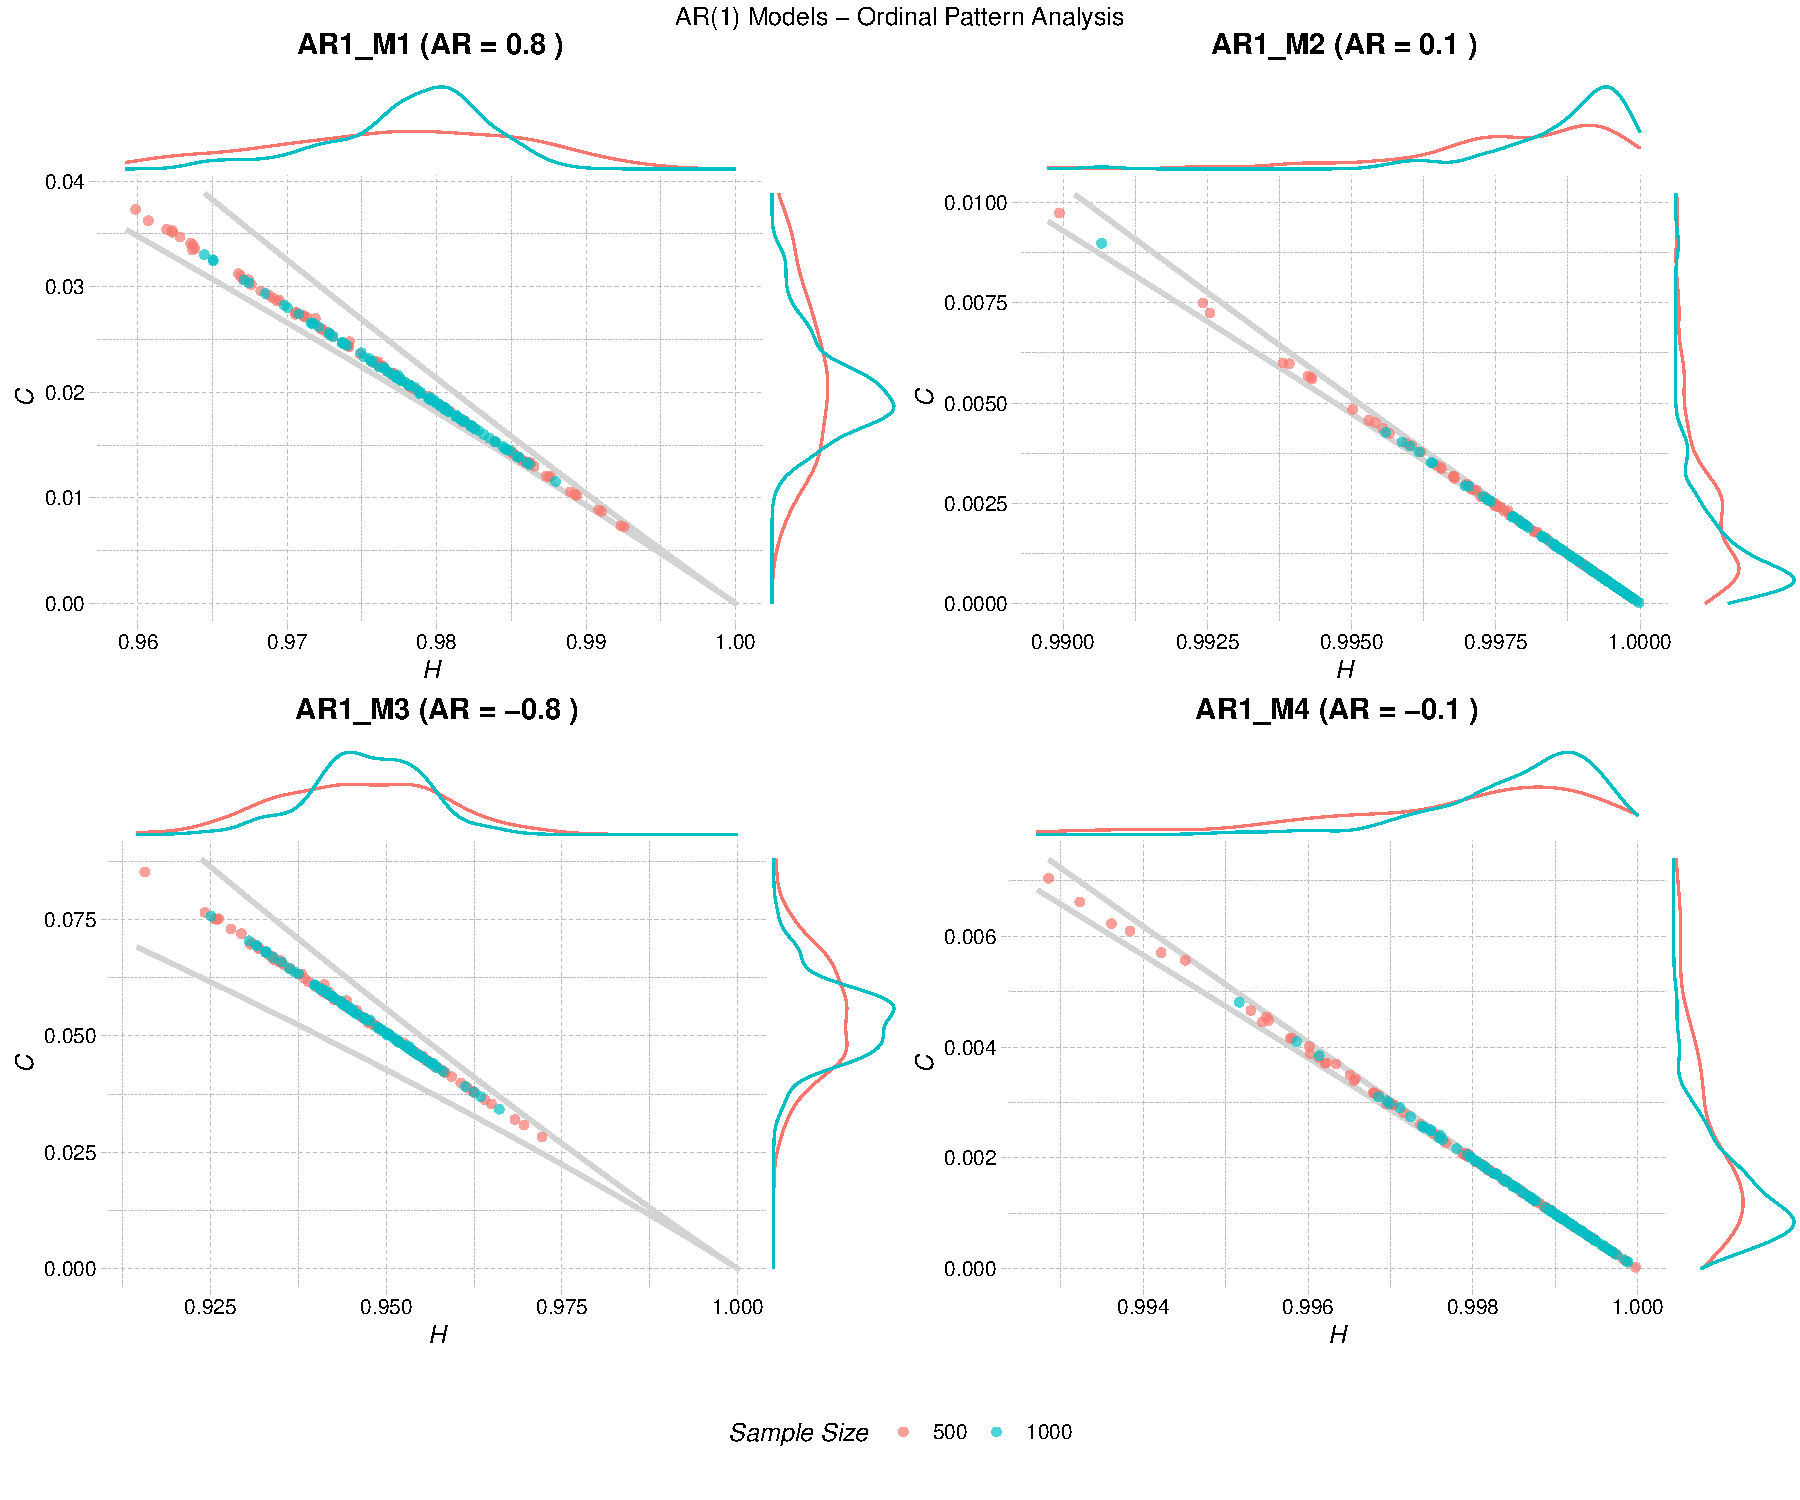
\includegraphics[width=0.9 \textwidth]{AR1_combined_analysis}
	\caption{$H \times C$ plane for AR(1) model}
	\label{fig:HC AR(1)}
\end{figure}	

\begin{figure}[H]
	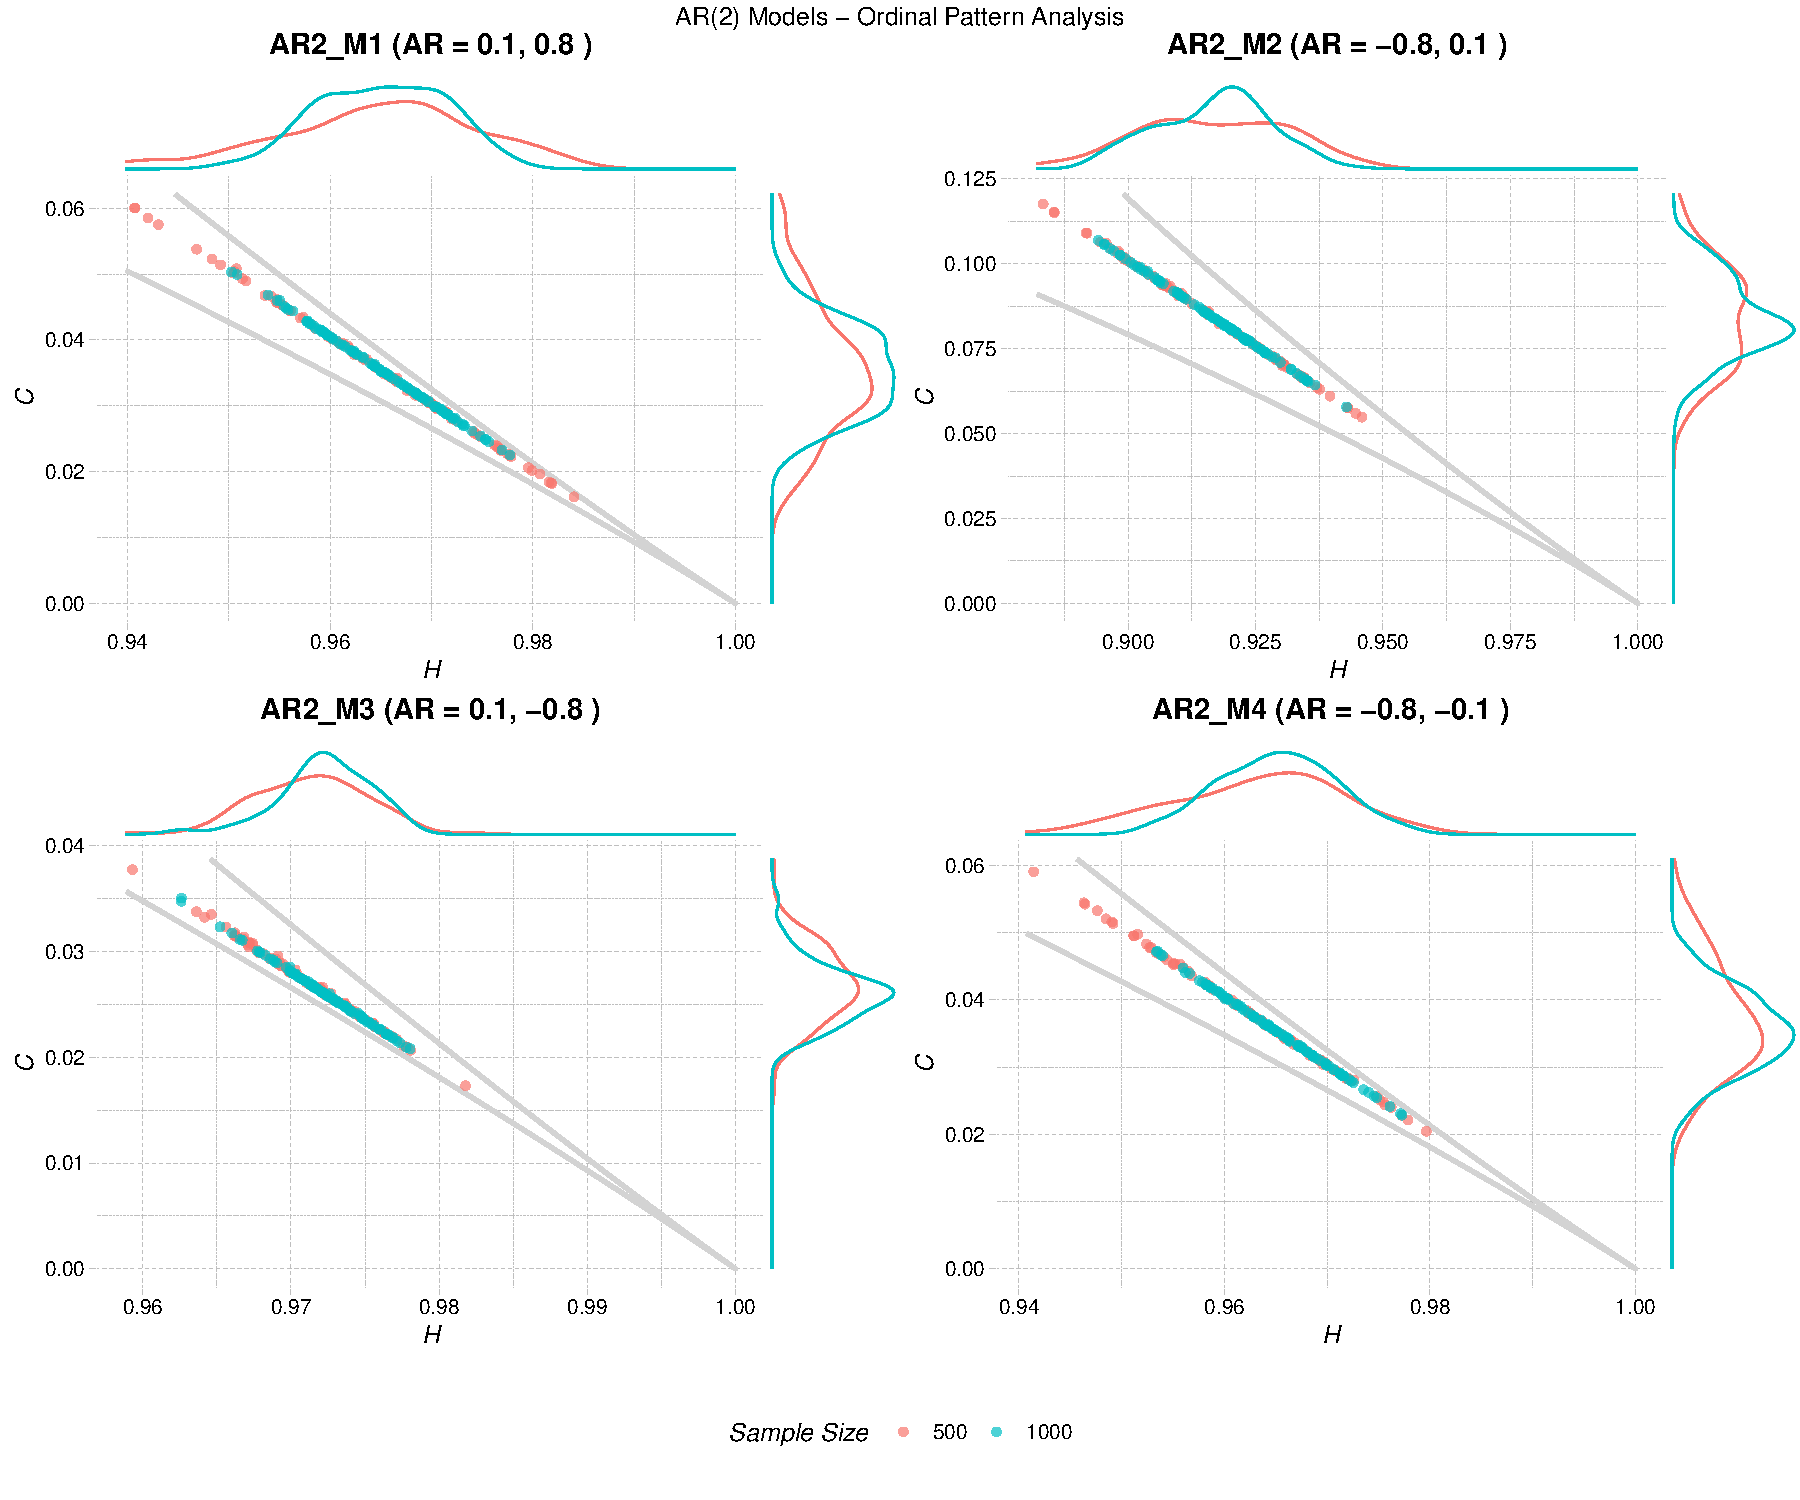
\includegraphics[width=0.9 \textwidth]{AR2_combined_analysis}
	\caption{$H \times C$ plane for AR(2) model}
	\label{fig:HC AR(2)}
\end{figure}

\begin{figure}[H]
	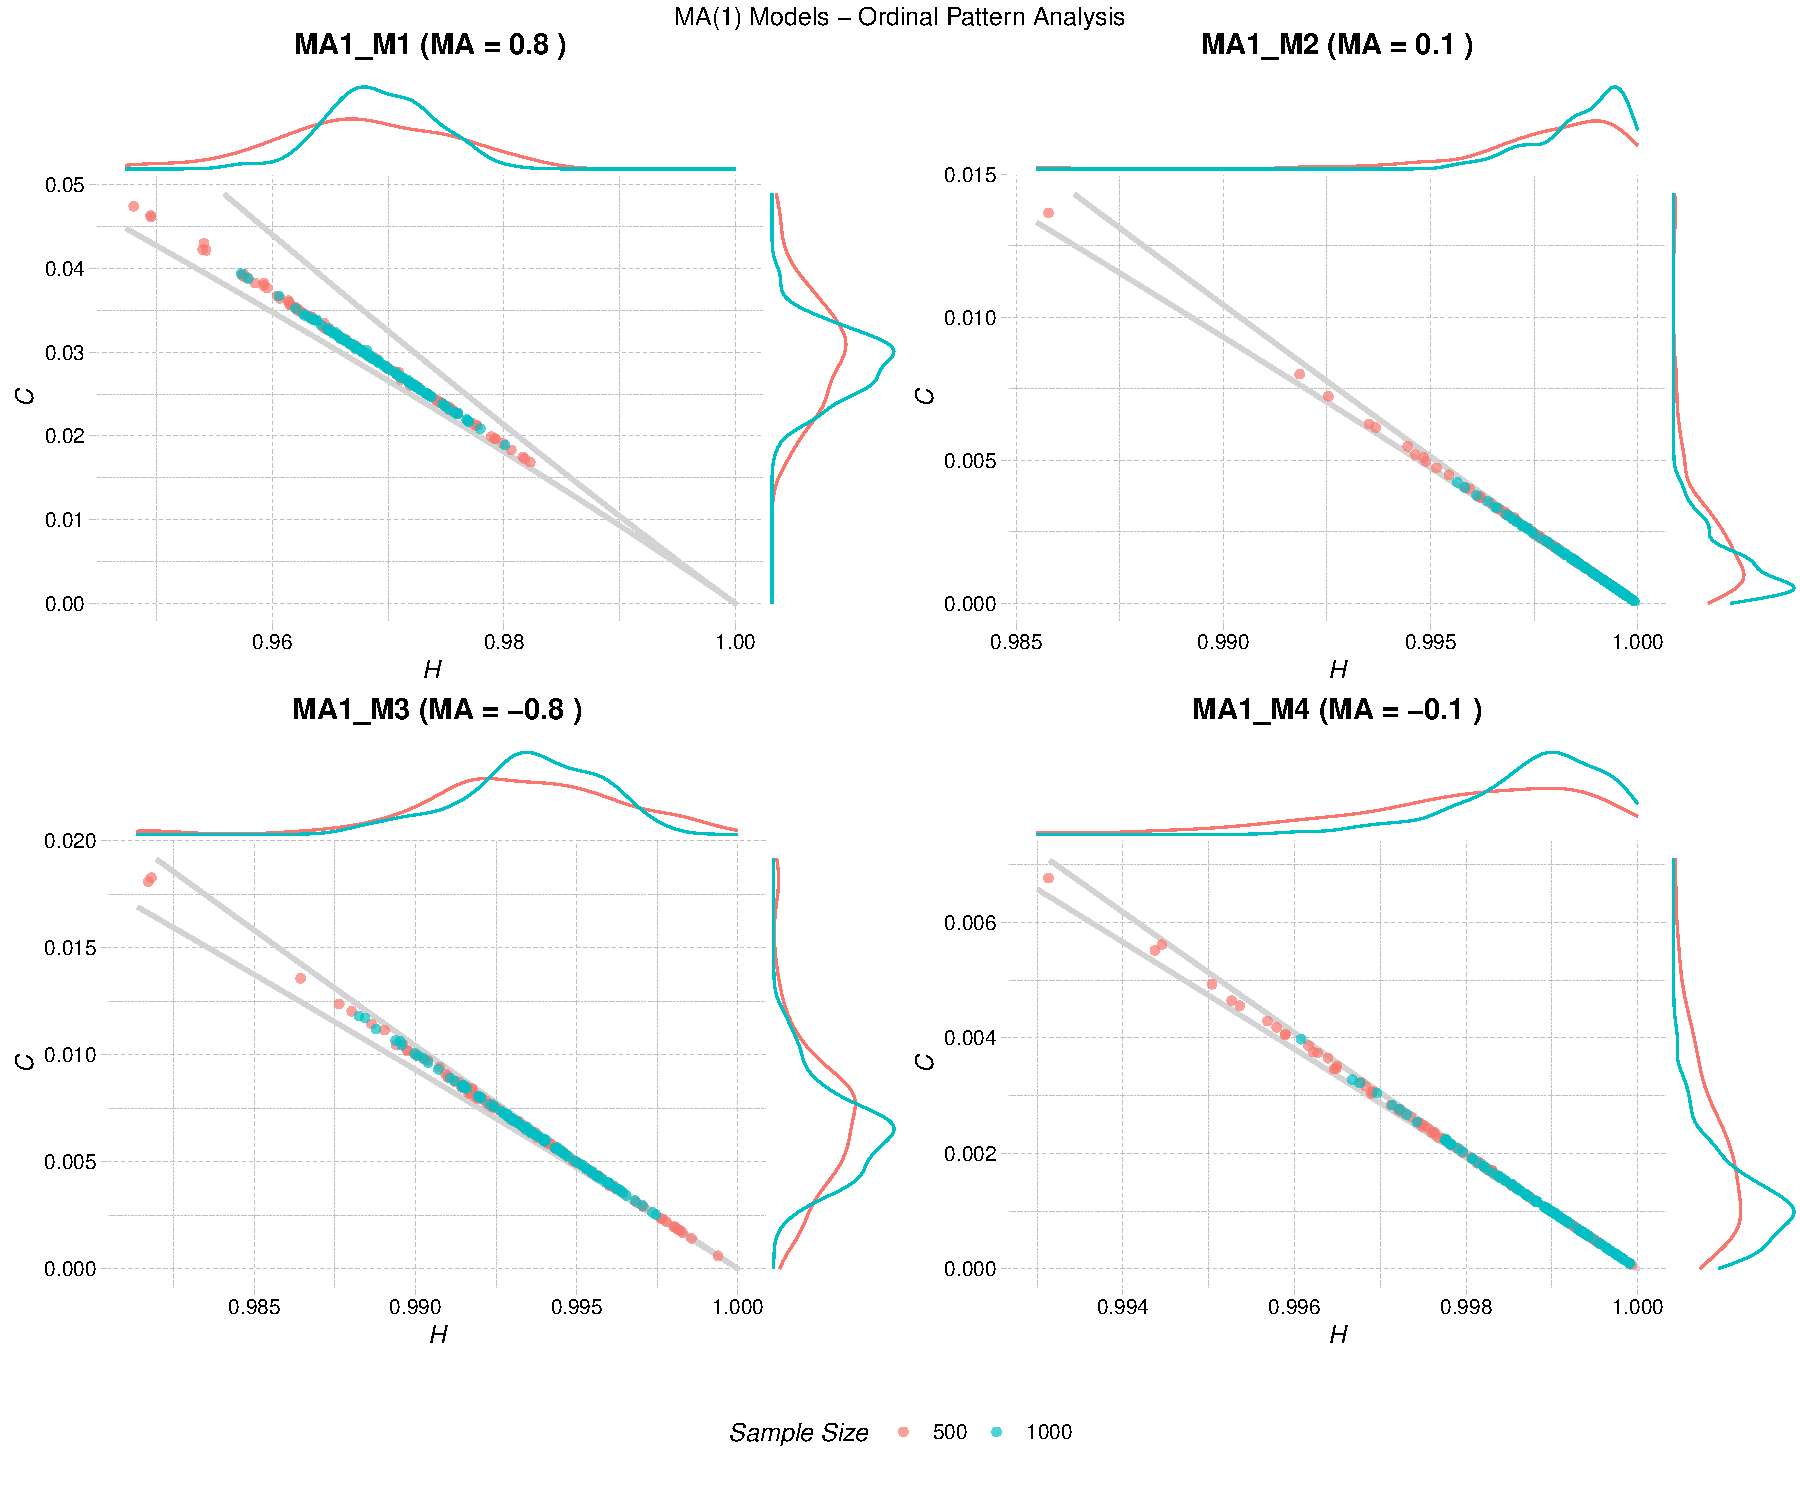
\includegraphics[width=0.9 \textwidth]{MA1_combined_analysis}
	\caption{$H \times C$ plane for MA(1) model}
	\label{fig:HC MA(1)}
\end{figure}

\begin{figure}[H]
	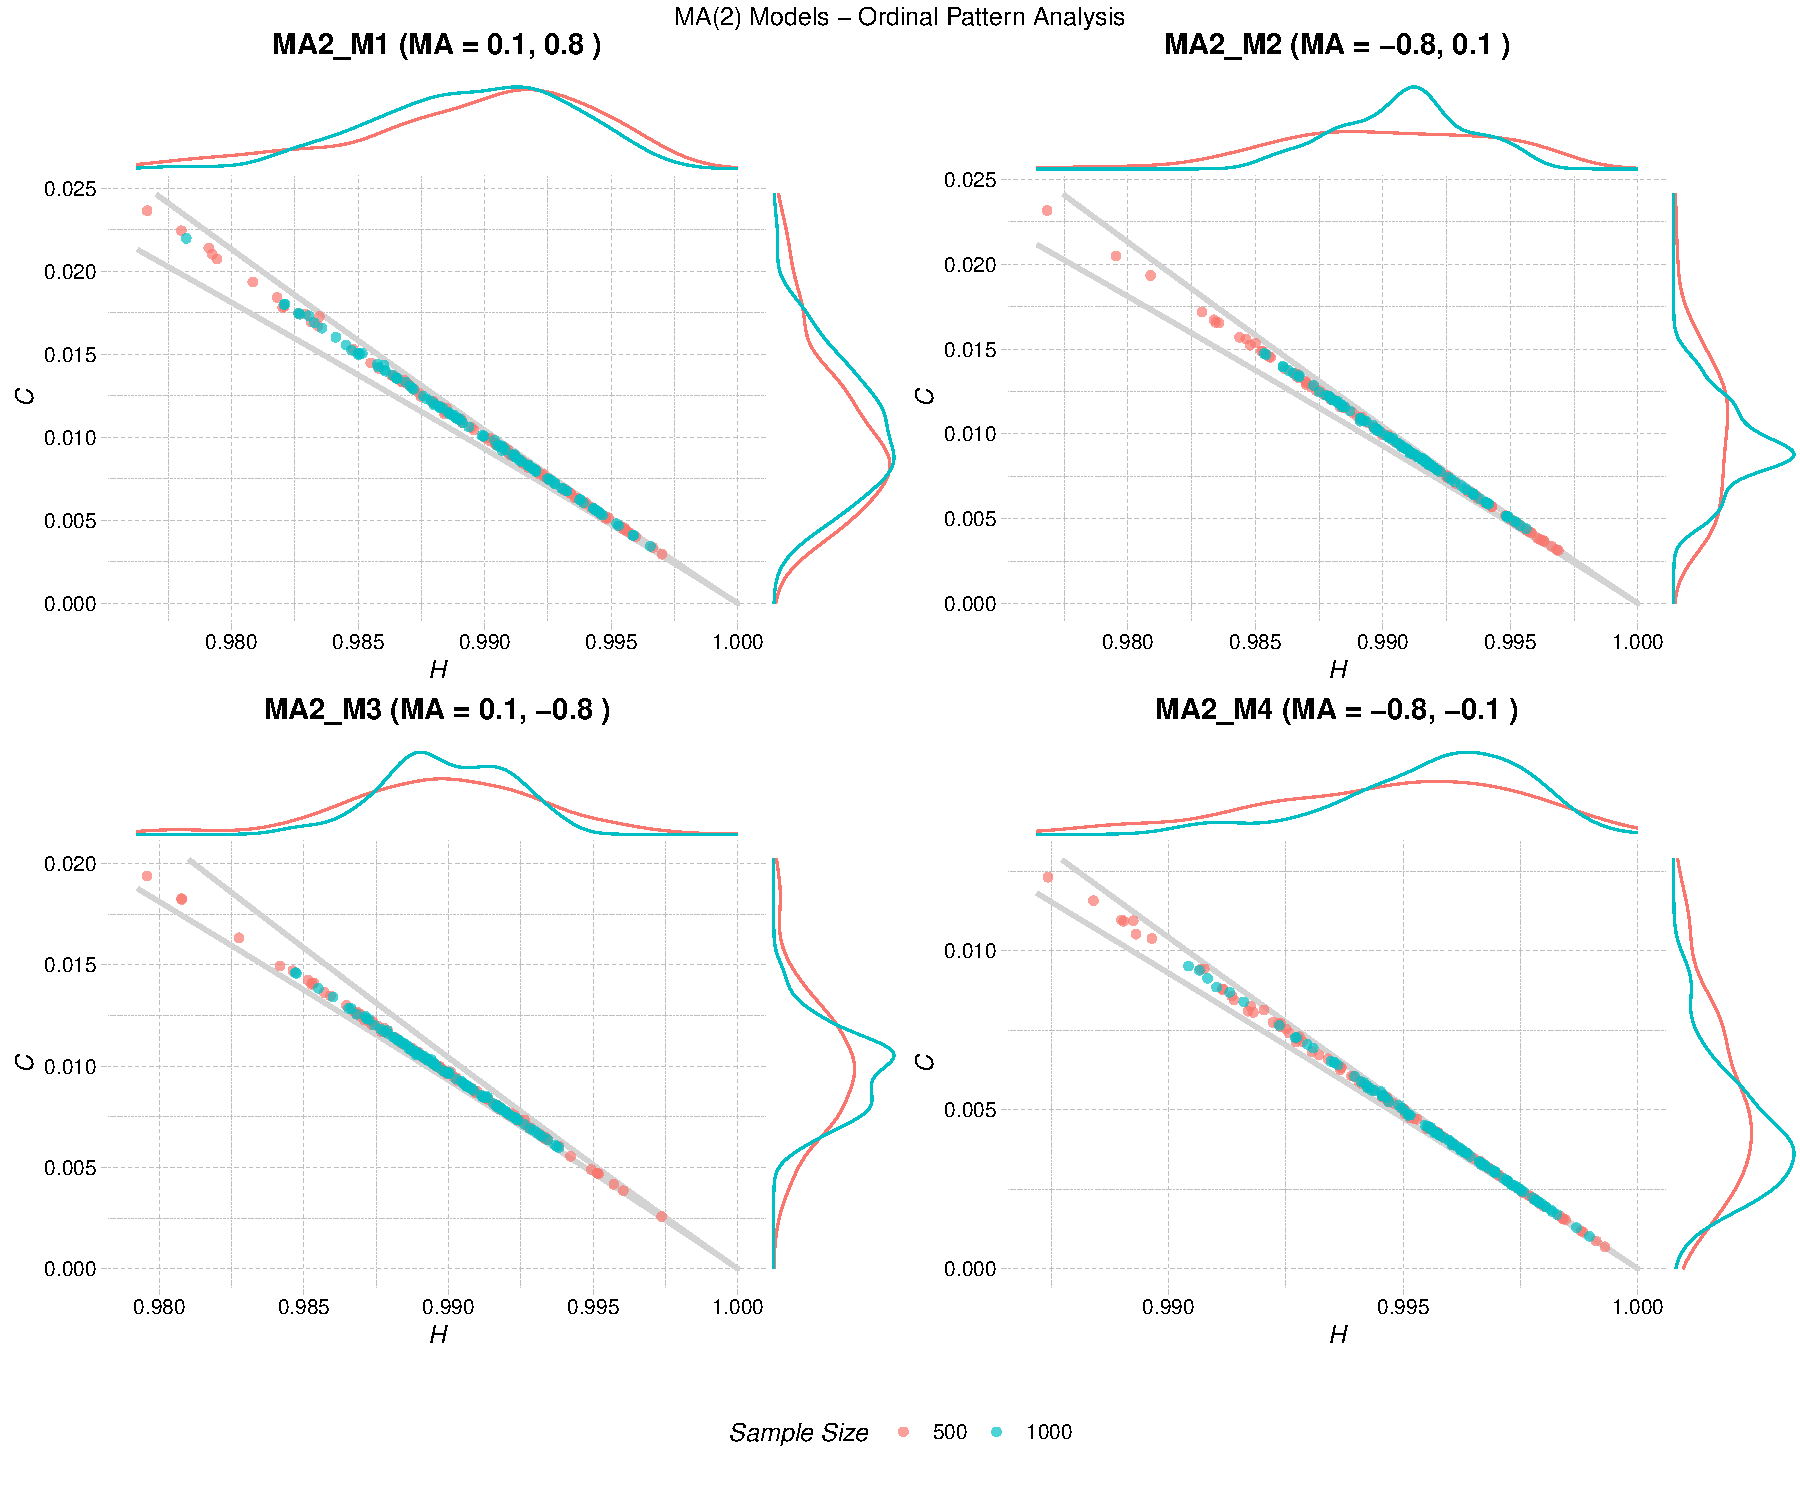
\includegraphics[width=0.9 \textwidth]{MA2_combined_analysis}
	\caption{$H \times C$ plane for MA(2) model}
	\label{fig:HC MA(2)}
\end{figure}			
	
\begin{figure}[H]
	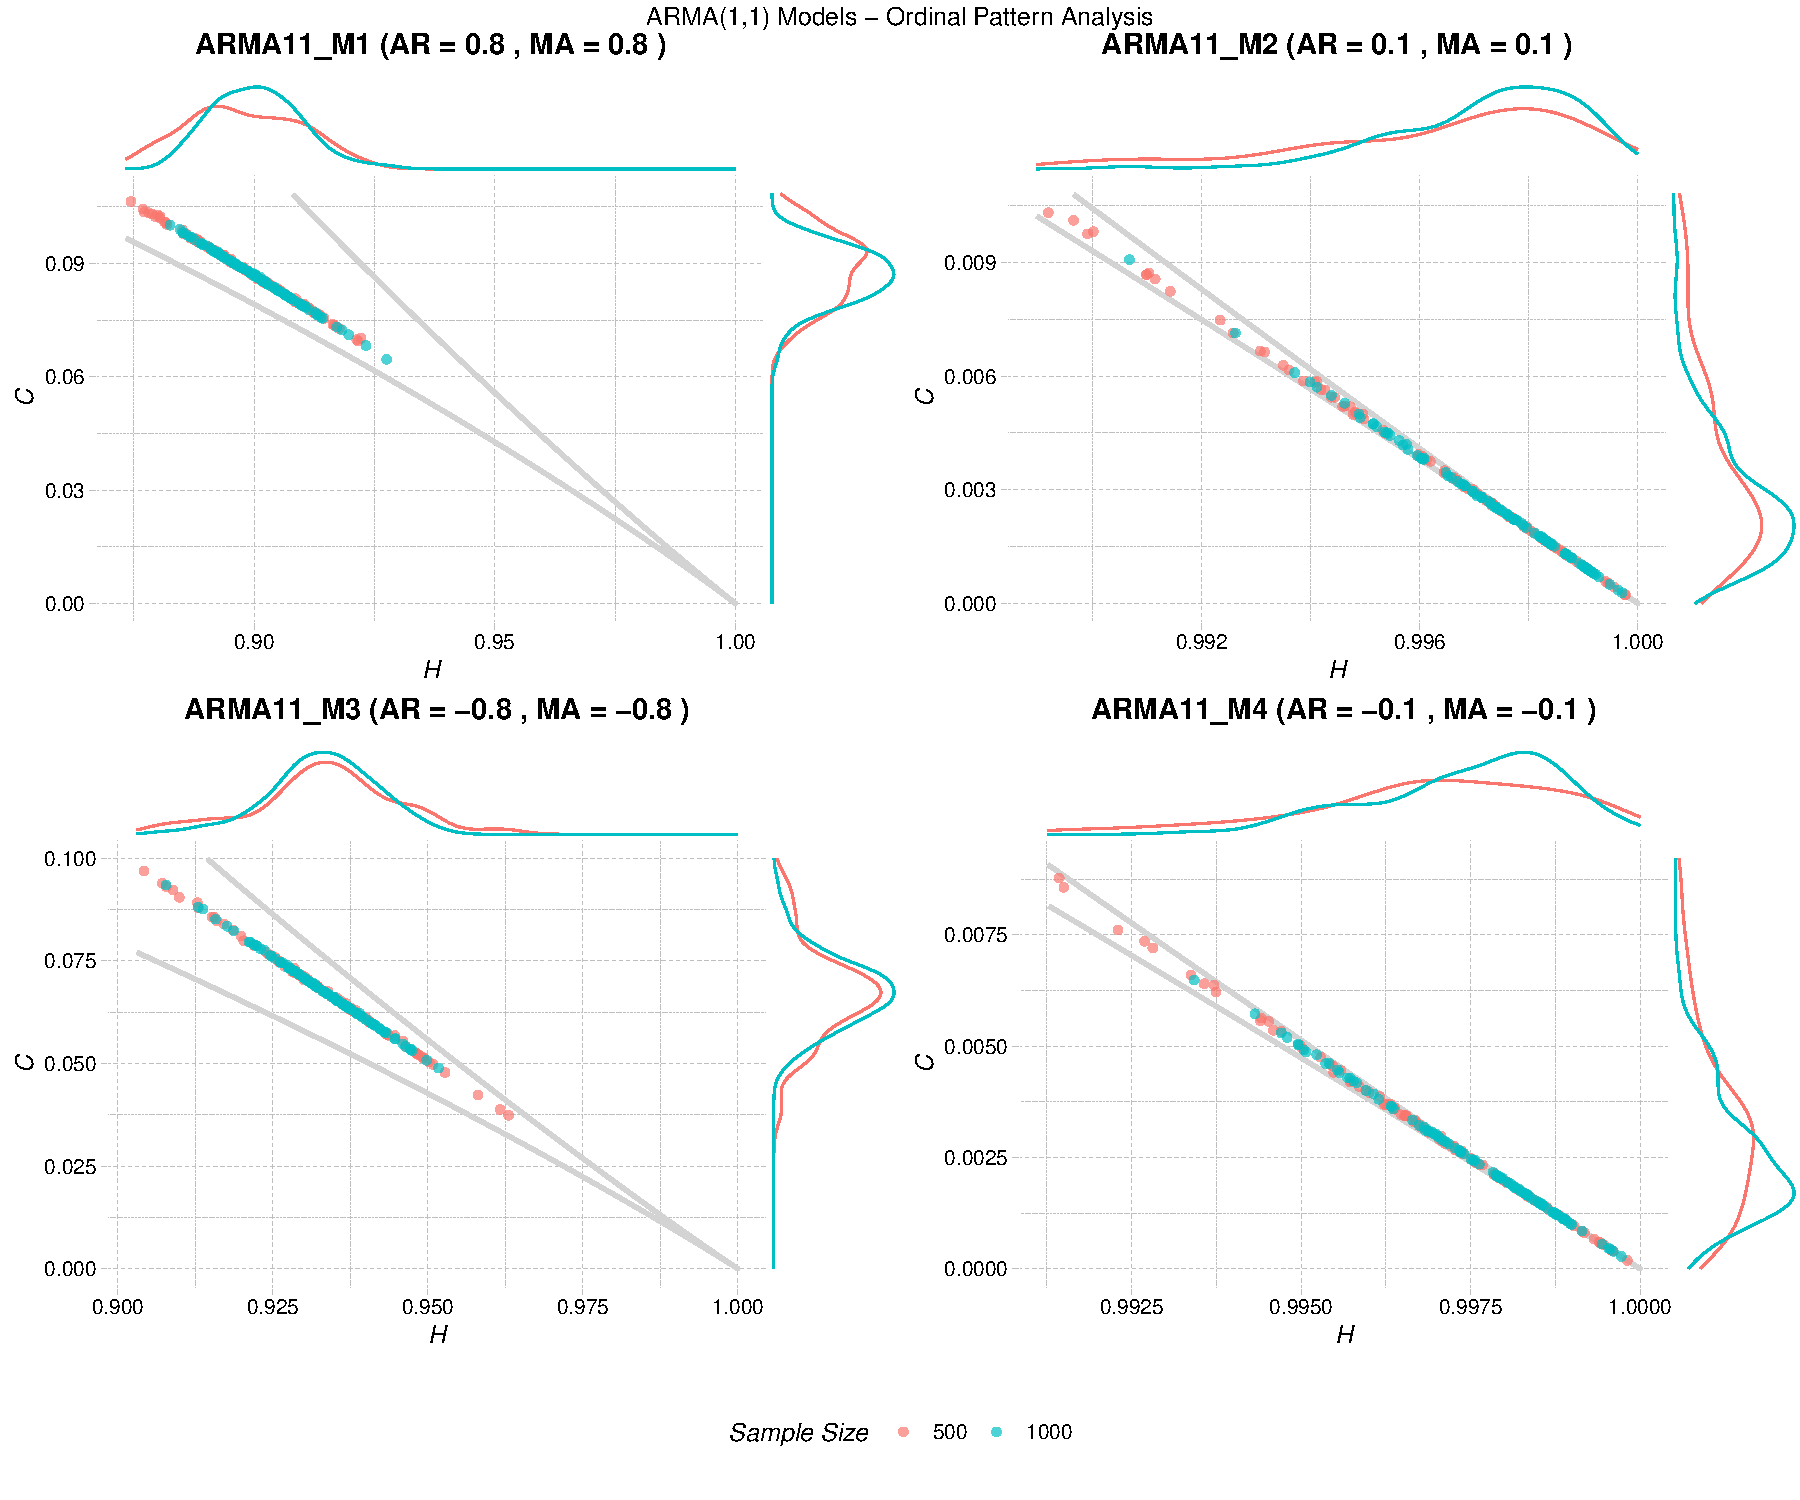
\includegraphics[width=0.9 \textwidth]{ARMA11_combined_analysis}
	\caption{$H \times C$ plane for ARMA(1,1) model}
	\label{fig:HC ARMA(11)}
\end{figure}	

\begin{figure}[H]
	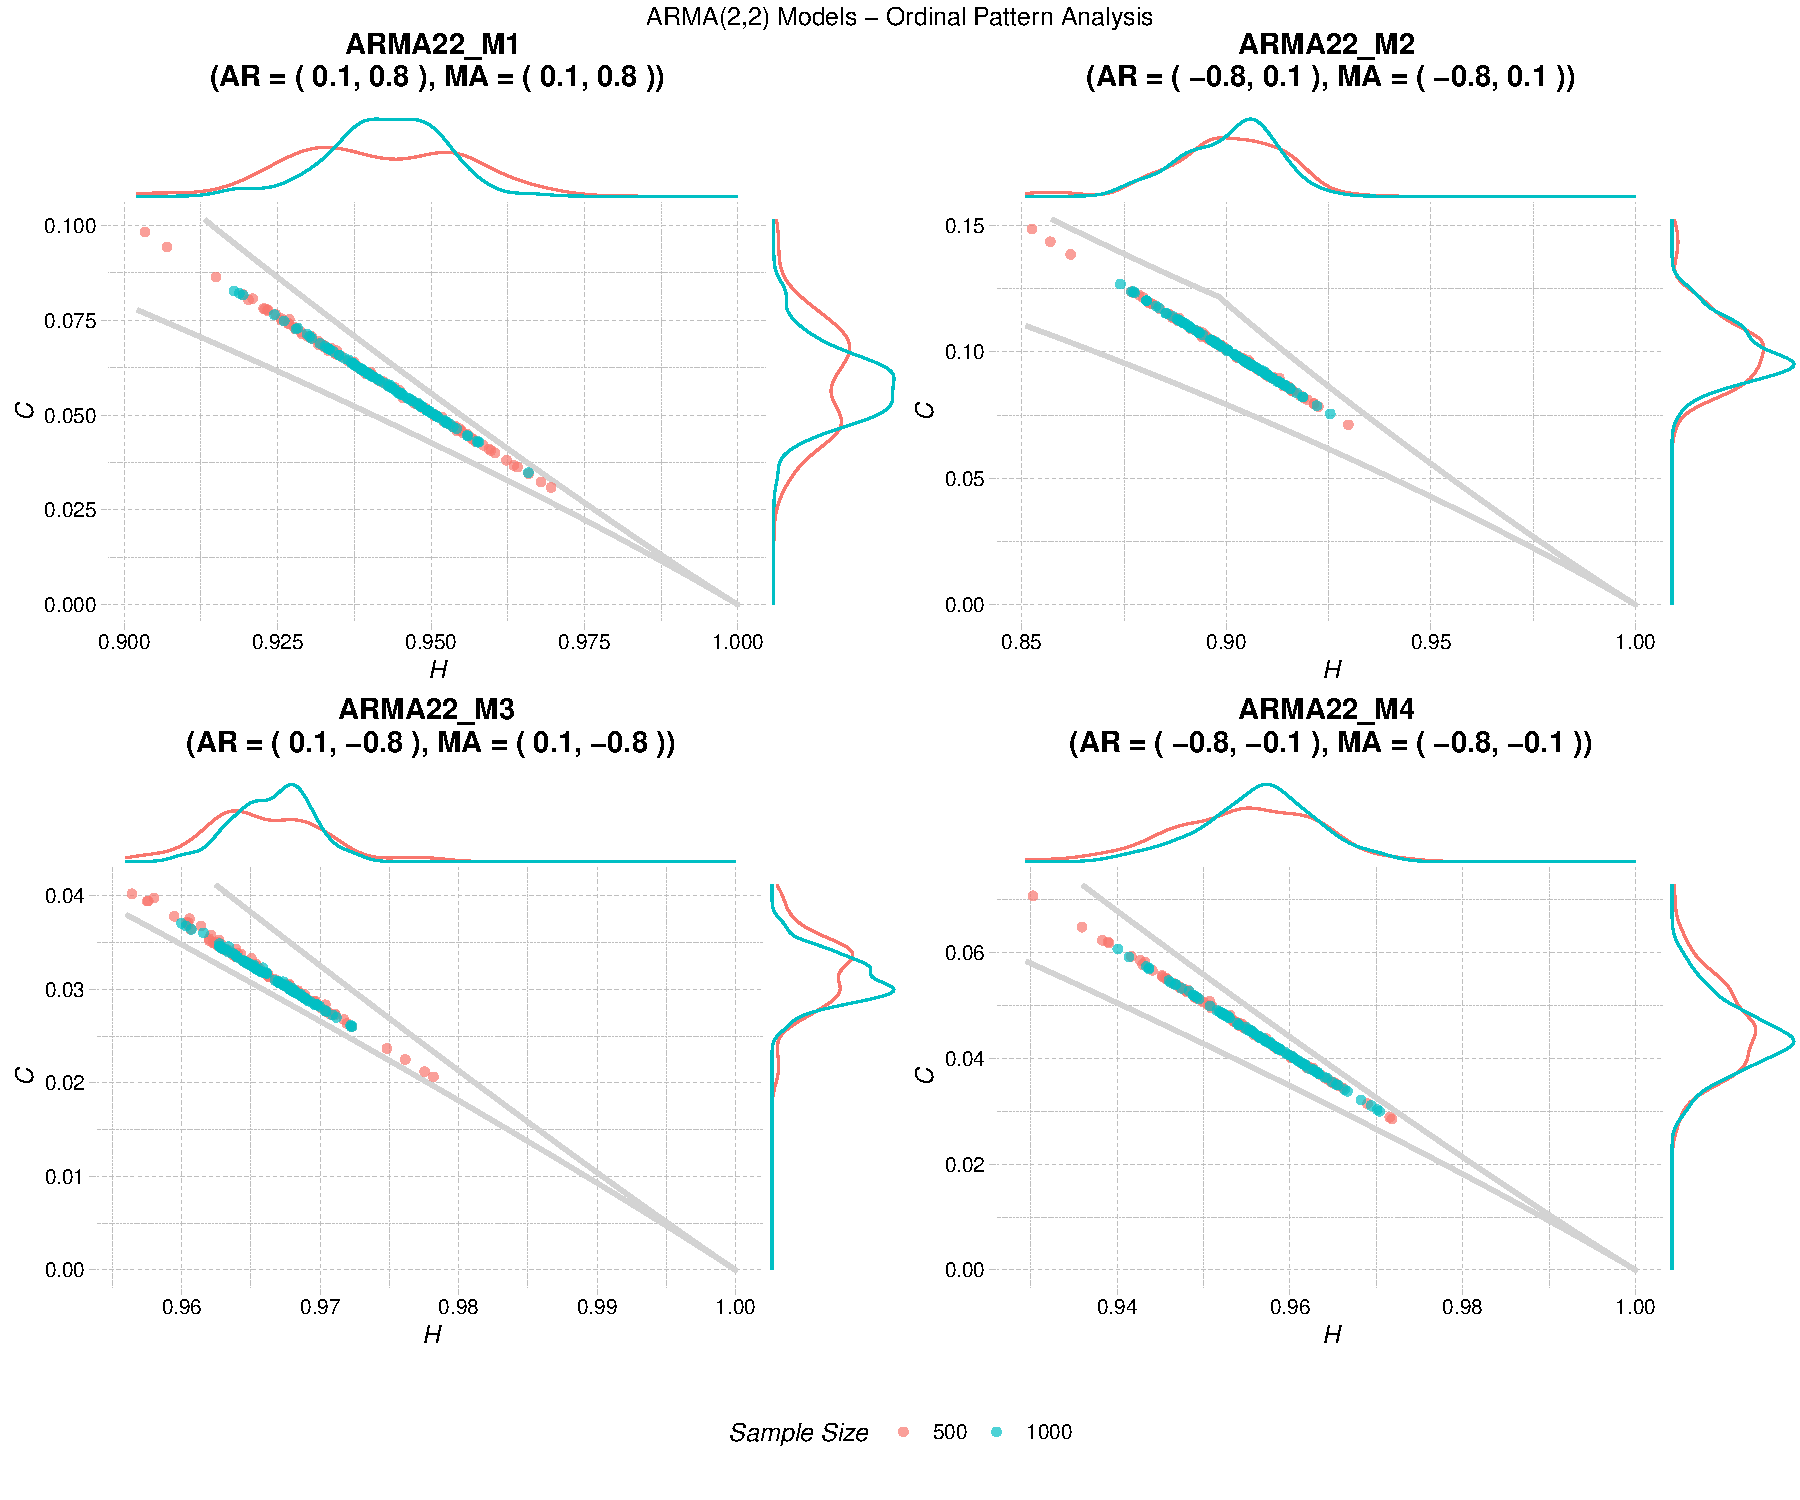
\includegraphics[width=0.9 \textwidth]{ARMA22_combined_analysis}
	\caption{$H \times C$ plane for ARMA(2,2) model}
	\label{fig:HC ARMA(22)}
\end{figure}


The results from the entropy–complexity analysis across AR1, AR2, MA1, MA2, ARMA(1,1), and ARMA(2,2) models reveal distinct clustering and spread patterns. These results provide key insights into the structural effects of different time series model classes and parameter variation.

For the AR1 models, series with stronger positive or negative coefficients exhibit lower entropy and higher complexity. In contrast, smaller coefficients allow greater entropy variation. In all cases, estimates become more precise with larger sample sizes.

AR2 models produce a wider spread in the entropy–complexity plane. This reflects the richer dynamics possible with two autoregressive lags. However, stationary parameter values remain within a consistent range of complexity.

The MA1 and MA2 analyses further demonstrate that moving average structure drives most realizations toward lower complexity. Entropy is also tightly controlled, especially for stronger coefficients. This reveals the smoothing and memory-limiting role of moving average behavior.

The ARMA(1,1) and ARMA(2,2) joint models combine these mechanisms. As a result, they produce denser, but still distinct, groupings in the ($H \times C$) diagram as both AR and MA parameters interact.

Overall, the increase in sample size reduces spread and enhances the reliability of entropy and complexity estimates. This comparative analysis shows how model order and parameter values directly influence the diversity and location of points in the entropy–complexity space. These results support the use of entropy and complexity for both identification and clustering of time series dynamics.
	
%	\bibliography{../BearingFaultDiagnosis}
	
\end{document}

